\documentclass[11pt]{scrreprt}
\usepackage[T1]{fontenc}
\usepackage[utf8]{inputenc}
\usepackage[french]{babel}
\usepackage[scale=0.775]{geometry}
\usepackage{lmodern}
\usepackage[ilines]{scrpage2}
\usepackage[pdftex, bookmarks=true, hidelinks]{hyperref}
\usepackage{graphicx}
\usepackage{tocbibind}
\usepackage{chngcntr}
\usepackage{tabularx}
\usepackage{float}
\usepackage{scrhack}
\usepackage{ulem}
\usepackage{mdframed}

\tolerance=1
\emergencystretch=\maxdimen
\hyphenpenalty=10000
\hbadness=10000

\counterwithout{figure}{chapter}
\counterwithout{table}{chapter}
\pagestyle{scrheadings}

\usepackage[table]{xcolor}
\definecolor{lightgray}{gray}{0.9}
\let\oldtabularx\tabularx
\let\endoldtabularx\endtabularx
\renewenvironment{tabularx}{\rowcolors{2}{white}{lightgray}\oldtabularx}{\endoldtabularx}

\let\oldtabular\tabular
\let\endoldtabular\endtabular
\renewenvironment{tabular}{\rowcolors{2}{white}{lightgray}\oldtabular}{\endoldtabular}

% clear head and foot
\clearscrheadings
\clearscrplain
\clearscrheadfoot

\cefoot[\textsc{Mighty Beards Studio}{\textsc{Mighty Beards Studio}}
\cofoot[\textsc{Mighty Beards Studio}{\textsc{Mighty Beards Studio}}
\lefoot[]{}
\lofoot[]{}
\refoot[\thepage]{\thepage}
\rofoot[\thepage]{\thepage}

\begin{document}

    \renewcommand{\labelitemi}{$\bullet$}
    \renewcommand{\labelitemii}{$\circ$}
    %%%%%% TITLE PAGE %%%%%%%%%%%%%%%%%%%


    %%%%%% TITLE PAGE %%%%%%%%%%%%%%%%%%%
    \begin{titlepage}
        \begin{center}
            ~\\[1.5cm]
            
\includegraphics[width=7.5cm]{images/blitzlogo.png}
            ~\\[1.5cm]

            %\textsc{\LARGE Mighty Beards Studio}\\[1.5cm]

            \textsc{\Large Projet d'AAE}\\[0.5cm]

            % Title
            \rule{\textwidth}{1pt} \\[0.4cm]
            { \bfseries \Huge{Blitz}\\ \Large{Clone du jeu Wazabi}\\[0.4cm]}

            \rule{\textwidth}{1pt} \\[1.5cm]

            % Authors
            \textsc{Javier Lethé - Matteo Taroli - Przemyslaw Gasinski}

            \vfill

            {\large \today}
            \vfill
        \end{center}
    \end{titlepage}
    \pagenumbering{gobble}
    \tableofcontents
    \pagebreak
    \pagenumbering{arabic}

    \setlength{\parskip}{3mm}
    %	#	#	#	#	#	#	#	#	#	#	#	#	#	#	#	#	# Document

    \chapter{Introduction}
    Wasabi est un jeu de dés et de cartes dont le but est de se débarrasser de tous ses dés. Nous avons dû, dans le cadre du cours de mise en situation professionnelle, implémenter ce jeu durant la semaine 13.

    Un des buts de ce projet étant de se rapprocher le plus possible de l'expérience professionnelle, certaines contraintes nous ont été imposées. Entre autres, le projet devait être développé en utilisant les technologies EJB et JSP, avec la possibilité d'utiliser d'autres technologies telles que Bootstrap, JavaScript et Ajax. Il nous a aussi été demandé de procéder de manière itérative, ce que nous avons fait en procédant par Usecase. Enfin, nous étions divisés en groupes de 4, qui ont été formés par les chefs d'équipe sur base de CV anonymes.

    Nous avons divisé le travail de la manière suivante: deux personnes se sont concentrées sur le back-end (la partie EJB) et deux sur le front-end (JSP). Malheureusement, un membre du groupe a décidé d'arrêter le projet en cours de route. De ce fait, nous avons dû re-distribuer afin de pouvoir continuer à avancer.

    Le délai assez court pour réaliser ce projet à trois ne nous a malheureusement pas permis de rendre un travail aussi propre que nous l'aurions souhaité. Par exemple, nous avons pensé à implémenter des patrons de conception supplémentaires par exemple pour la gestion des effets de cartes, améliorer l'interface ou encore un timer permettant de lancer le jeu après 30 secondes.
    Dans la suite de ce rapport, nous allons présenter les détails du programme développé.

    \chapter{Analyse}
    \section{Diagramme de navigation}
    Le parcours de l'utilisateur dans \textsc{Blitz} se fait selon le diagramme suivant :

    \begin{table}[H]
        \centering
        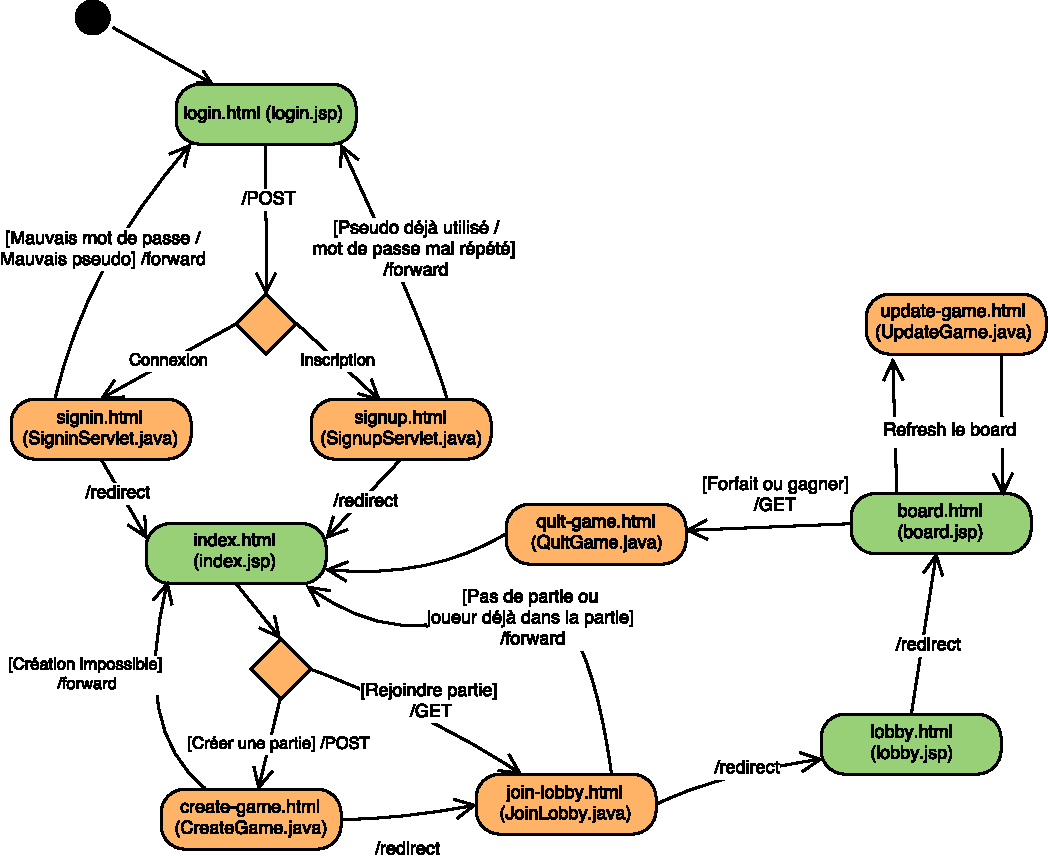
\includegraphics[width=\textwidth]{images/diag-nav.pdf}
        \caption{Diagramme de navigation}
    \end{table}

    \section{Scénario nominal \og Rejoindre une partie\fg}

    L'utilisateur étant déjà connecté, il rejoint une partie selon le scénario suivant :

    \begin{table}[H]
        \begin{tabularx}{\textwidth}{X|X}
            1. Le joueur clique sur le bouton \og Rejoindre une partie \fg{} & \\
            & 2. Le système vérifie si une partie est déjà lancée \\
            3.a [Une partie est en cours de lancement] & \\
            & a.1 Le système envoie le joueur vers le lobby.\\
            & a.2 Une fois que le nombre minimal de joueur est atteint, le jeu est lancé\\
            3.b [Aucune partie n'est en cours] & \\
            & b.1 Le système informe le joueur et le renvoie vers la page de création de jeu. \\
            b.2 Le joueur crée une partie & \\
            & b.3 Le système envoie le joueur vers le lobby. \\
            & b.4 Une fois que le nombre minimal de joueur est atteint, le jeu est lancé\\
            3.c [Une partie est déjà en cours de jeu] & \\
            & c.1 Le système ne permettant de lancer qu'une partie à la fois, il informe le joueur et le renvoie vers la page d'accueil.\\
        \end{tabularx}
    \end{table}

    \section{Tests Fonctionnels}
    \section{Connexion}
    \begin{table}[H]
        \begin{tabularx}{\textwidth}{X|X}
            1. Cliquer sur le bouton \og Connexion / Inscription\fg{} situé en haut à droite. & \\
            & 2. Un popup apparait proposant de s'inscrire ou de se connecter. \\
            3. Dans la partie de droite, entrer \og ol\fg{} comme nom d'utilisateur et \og ol \fg{} comme mot de passe. & \\
            & 4. Le système vérifie que l'utilisateur existe et que le mot de passe est correct et renvoie le joueur sur la page d'accueil. \\
            5. Cliquer sur le bouton \og Déconnexion\fg{}. & \\
            6. Cliquer à nouveau sur le bouton \og Connexion / Inscription\fg{}. & \\
            & 7. Le popup réapparait \\
            8. Dans la partie de droite, entrer \og ol\fg{} comme nom d'utilisateur et \og mauvaisMdp \fg{} comme mot de passe. & \\
            & 9. Le système vérifie que l'utilisateur existe et que le mot de passe est correct et affiche l'erreur \og Nom d'utilisateur ou mot de passe incorrect\fg{} et reste sur le popup.\\
        \end{tabularx}
    \end{table}
    \section{Création de partie}
    \begin{table}[H]
        \begin{tabularx}{\textwidth}{X|X}
            1. En partant de la page d'accueil, cliquer sur le bouton \og Créer une partie\fg{}. & \\
            & 2. Un popup apparait permettant d'entrer le nom de la partie.\\
            3. Entrer \og test\fg{} en tant que nom de partie. & \\
            4. Cliquer sur le bouton \og OK\fg{}. & \\
            & 5.Le système renvoie vers le lobby de la partie. \\
            6.Attendre d'autres joueurs et joueur. & \\
        \end{tabularx}
    \end{table}

    \section{Jeu}
    \begin{table}[H]
        \begin{tabularx}{\textwidth}{X|X}
            1. Attendre que ce soit
        \end{tabularx}
    \end{table}

    \chapter{Manuels}
    \section{Manuel d'installation}

    \section{Manuel d'utilisation}
    \subsection{Comment accéder au jeu?}
    Pour jouer sur une machine locale, tapez dans le browser \og \url{localhost:8080/Blitz}\fg{} (sans les guillemets).

    Une fois connecté, vous arrivez sur l'écran suivant:

    [ECRAN D ACCEUIL] (screenshot)

    \subsection{Comment créer une partie?}
    Pour lancer une partie, il vous suffit de cliquer sur créer une partie.
    Si \textbf{aucune partie n'a été créée}, une pop-up apparaitra alors pour que vous donniez un nom à la partie. Après ça, vous voilà redirigé vers le lobby.

    Si une \textbf{partie est déjà créée}, et que vous ne \textbf{pouvez pas la rejoindre} (ce qui arrive si la partie est déjà en cours ou si le nombre de joueurs maximum est déjà atteint), le bouton est désactivé et vous empêche donc de cliquer dessus.

    \subsection{Comment rejoindre une partie?}
    Pour rejoindre une partie, cliquez sur le bouton correspondant sur la page d'accueil.

    Si une partie est \textbf{en attente de joueurs supplémentaires}, vous serez redirigé vers le lobby de cette partie.

    Si vous ne pouvez pas rejoindre la partie créée (\textbf{aucune partie}, partie \textbf{en cours} ou le \textbf{nombre de joueurs maximum est atteint}), le bouton est désactivé.

    \subsection{Comment lancer une partie?}
    Une fois dans la lobby, la partie se lance automatiquement une fois le nombre minimum de joueur atteint. Une fois ce nombre atteint, tous les joueurs sont redirigés vers la page de jeu.

    \subsection{Comment se déroule le tour de jeu?}

    \chapter{Conclusion}

\end{document}
